\documentclass[11pt]{article}

\usepackage[margin=1in]{geometry}
\usepackage{booktabs}
\usepackage{array}
\usepackage{tikz}
\usetikzlibrary{arrows.meta, positioning}

\title{Milestone: Inductive Graph-Based Imputation for Sparse Self-Tracked Women's Health Data}
\author{%
  Julia Isaac \quad Zoe Brickley \quad Ashley Vincent \\
  Department of Computer Science \\
  Stanford University \\
  Stanford, CA 94305 \\
  \texttt{\{juliai, zbrick, ashleyv1\}@stanford.edu} \\
}
\date{}

\begin{document}
\maketitle

\section{Milestone Summary}
Our project investigates whether graph-based imputation of self-reported
women's health data can improve downstream prediction tasks. With the
recent rise of women's health apps, users can self-report their own data,
which comes with inherent noise and sparsity (e.g. a person may not record symptoms
or events every day). In our milestone, we implement an end-to-end synthetic test bed for graph-based
imputation while access to our planned test dataset (mcPHASES) is pending.

\section{Dataset Description and Processing}
Our synthetic data simulator uses the same set of features as the data
generator accompanying prior work by Liu et al. \cite{liu2019pregnancy}.
The simulator generates one 24-day cycle for each synthetic patient. Each
day contains six binary features:
\begin{itemize}
    \item unprotected, protected, or withdrawal sex;
    \item happy, neutral, or sad emotion.
\end{itemize}
Sex and emotion entries are sampled independently each day. The simulated
pregnancy label is derived from a fixed cycle-day fertility curve,
sex-category risk weights, an emotion multiplier, patient fertility
susceptibility, and random noise.

Each patient is assigned stable latent tendencies for sex activity,
emotion-reporting frequency, feature-category preferences, and fertility
susceptibility. These traits affect that patient's generated event
patterns and pregnancy risk. The \texttt{structure-strength} parameter
controls how strongly the traits influence generation. These are explicit
simulator assumptions, not clinical factors.

By default, the experiment randomly hides 30\% of days. When a day is
hidden, all six feature values---including zeros---are treated as
unreported. Original values and an observation mask are retained so
reconstruction can be evaluated against ground truth. Patients are split
into fit, validation, and test groups before fitting. The imputer uses
the fit group; validation observations are used for model selection; test
patients are held out for final evaluation.
\begin{figure}[htbp]
\centering
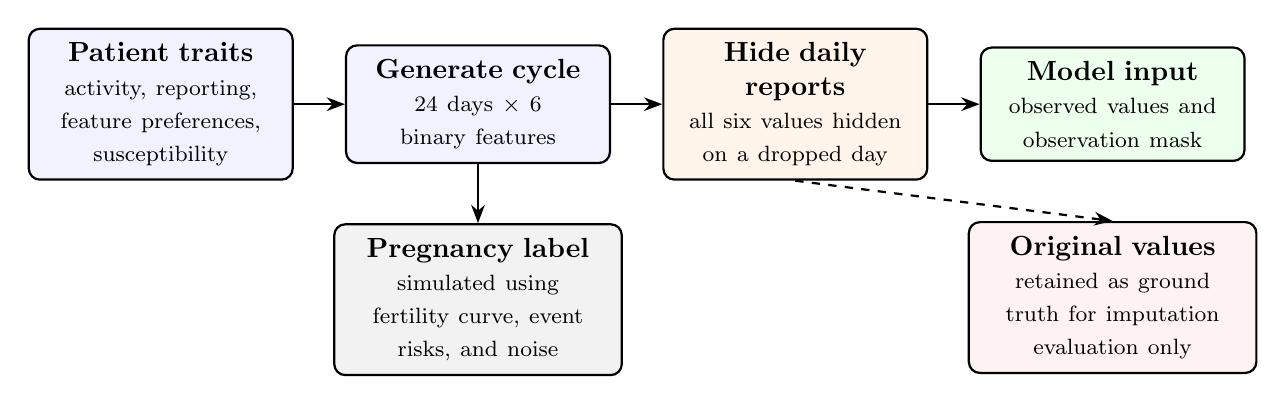
\begin{tikzpicture}[
    >=Stealth,
    box/.style={
        draw, rounded corners, thick, align=center,
        text width=3.0cm, minimum height=1.05cm, inner sep=5pt
    },
    arrow/.style={->, thick}
]
\node[box, fill=blue!5] (traits) {
    \textbf{Patient traits}\\
    \footnotesize activity, reporting, feature preferences, susceptibility
};
\node[box, fill=blue!5, right=0.65cm of traits] (cycle) {
    \textbf{Generate cycle}\\
    \footnotesize 24 days $\times$ 6 binary features
};
\node[box, fill=orange!8, right=0.65cm of cycle] (mask) {
    \textbf{Hide daily reports}\\
    \footnotesize all six values hidden on a dropped day
};
\node[box, fill=green!7, right=0.65cm of mask] (input) {
    \textbf{Model input}\\
    \footnotesize observed values and observation mask
};

\node[box, fill=gray!10, below=0.75cm of cycle, text width=3.3cm] (label) {
    \textbf{Pregnancy label}\\
    \footnotesize simulated using fertility curve, event risks, and noise
};
\node[box, fill=red!5, below=0.75cm of input, text width=3.3cm] (truth) {
    \textbf{Original values}\\
    \footnotesize retained as ground truth for imputation evaluation only
};

\draw[arrow] (traits) -- (cycle);
\draw[arrow] (cycle) -- (mask);
\draw[arrow] (mask) -- (input);
\draw[arrow] (cycle.south) -- (label.north);
\draw[arrow, dashed] (mask.south) -- (truth.north);
\end{tikzpicture}
\caption{Synthetic data generation and masking. Missing values are
represented separately from observed zeros. The original values are
retained for evaluation but are not given to the imputer.}
\label{fig:data}
\end{figure}

\section{Model Design and Metrics}

\subsection{Graph Autoencoder}

The imputer is a learned, self-supervised bipartite graph autoencoder.
It represents fit patients as patient nodes and each day/category
combination as a time-conditioned feature node. An observed positive
patient-feature value creates an edge. Feature-node representations combine
learned day and category embeddings.

Patient and feature nodes pass messages across observed patient-feature
edges. A learned inner-product decoder estimates the probability of each
patient-feature event. During training, some observed positive events are
temporarily withheld for reconstruction; known observed zeros are sampled
as negative examples. Truly unobserved values do not create graph edges
and are excluded from the reconstruction loss. The decoder is trained with
binary cross-entropy. Validation data is used for early stopping.

At inference, a new patient is encoded using visible events and information
from similar fit-patient nodes. Fit patients use leave-one-out neighbor
connections, while validation and test patients connect only to fit
patients. Pregnancy labels are not used to fit the imputer or construct
the graph.
\begin{figure}[htbp]
\centering
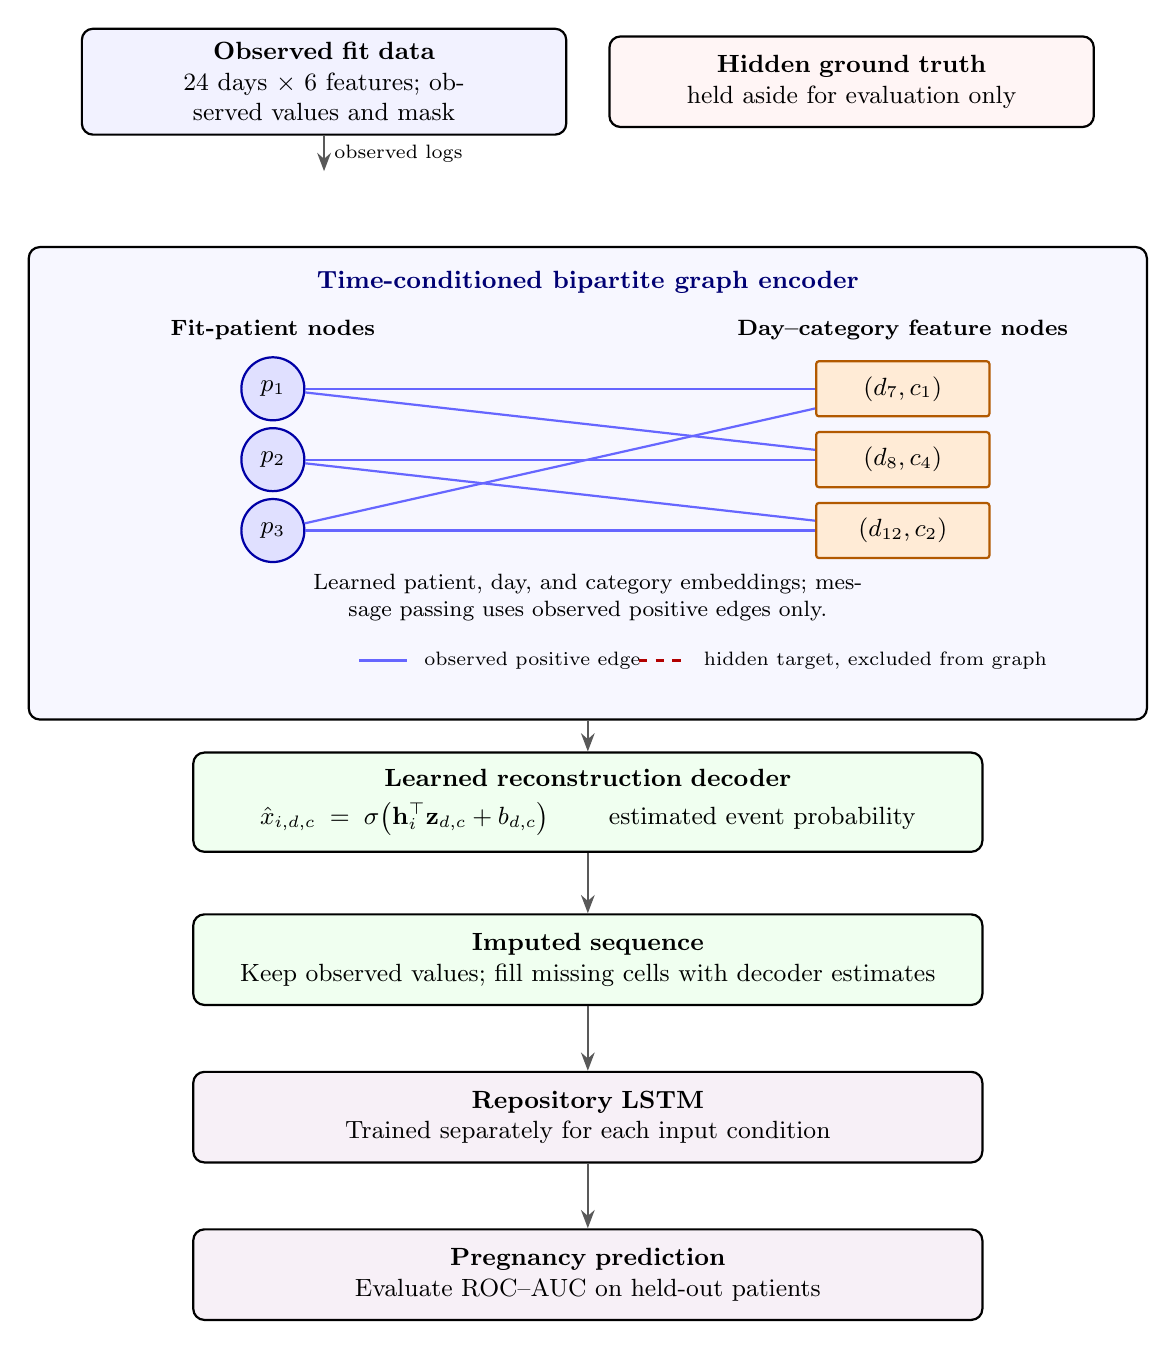
\begin{tikzpicture}[
    x=1cm,
    y=1cm,
    font=\small,
    >=Stealth,
    inputbox/.style={
        draw, rounded corners, thick, align=center,
        text width=5.8cm, minimum height=1.15cm, inner sep=5pt
    },
    stage/.style={
        draw, rounded corners, thick, align=center,
        text width=9.6cm, minimum height=1.15cm, inner sep=6pt
    },
    graphpanel/.style={
        draw, rounded corners, thick, fill=blue!3,
        minimum width=14.2cm, minimum height=6.0cm
    },
    patient/.style={
        circle, draw=blue!65!black, fill=blue!12, thick,
        minimum size=8mm, inner sep=1pt
    },
    feature/.style={
        rectangle, rounded corners=1pt, draw=orange!70!black,
        fill=orange!16, thick, minimum width=2.2cm,
        minimum height=7mm, inner sep=3pt
    },
    flow/.style={->, thick, draw=gray!70!black},
    observed/.style={-, thick, draw=blue!60},
    heldout/.style={-, thick, dashed, draw=red!70!black}
]

% Inputs. The ground-truth box is intentionally not connected to the model.
\node[inputbox, fill=blue!5] (input) at (-3.35,0) {
    \textbf{Observed fit data}\\
    24 days $\times$ 6 features; observed values and mask
};
\node[inputbox, fill=red!4] (truth) at (3.35,0) {
    \textbf{Hidden ground truth}\\
    held aside for evaluation only
};

% Bipartite graph panel.
\node[graphpanel] (graph) at (0,-5.1) {};
\node[font=\small\bfseries, text=blue!45!black] at (0,-2.55)
    {Time-conditioned bipartite graph encoder};
\node[font=\footnotesize\bfseries] at (-4,-3.15) {Fit-patient nodes};
\node[font=\footnotesize\bfseries] at (4,-3.15) {Day--category feature nodes};

% Patient nodes.
\node[patient] (p1) at (-4,-3.9) {$p_1$};
\node[patient] (p2) at (-4,-4.8) {$p_2$};
\node[patient] (p3) at (-4,-5.7) {$p_3$};

% Time-conditioned feature nodes.
\node[feature] (f1) at (4,-3.9) {$(d_7,c_1)$};
\node[feature] (f2) at (4,-4.8) {$(d_8,c_4)$};
\node[feature] (f3) at (4,-5.7) {$(d_{12},c_2)$};

% Observed positive patient-feature edges.
\draw[observed] (p1) -- (f1);
\draw[observed] (p1) -- (f2);
\draw[observed] (p2) -- (f2);
\draw[observed] (p2) -- (f3);
\draw[observed] (p3) -- (f1);
\draw[observed] (p3) -- (f3);

% Explanation and legend are kept below the graph nodes.
\node[font=\footnotesize, align=center, text width=11cm] at (0,-6.55) {
    Learned patient, day, and category embeddings; message passing uses
    observed positive edges only.
};
\draw[observed] (-2.9,-7.35) -- (-2.3,-7.35);
\node[font=\scriptsize, anchor=west] at (-2.2,-7.35) {observed positive edge};
\draw[heldout] (0.65,-7.35) -- (1.25,-7.35);
\node[font=\scriptsize, anchor=west] at (1.35,-7.35) {hidden target, excluded from graph};

% Observed data enters the graph. Original hidden values remain separate.
\draw[flow] (input.south) -- ++(0,-0.45)
    node[midway, right, font=\scriptsize] {observed logs};

% Decoder and downstream prediction stages.
\node[stage, fill=green!6] (decoder) at (0,-9.15) {
    \textbf{Learned reconstruction decoder}\\[1mm]
    $\hat{x}_{i,d,c} =
      \sigma\!\left(\mathbf{h}_i^\top
      \mathbf{z}_{d,c}+b_{d,c}\right)$
    \qquad estimated event probability
};
\draw[flow] (graph.south) -- (decoder.north);

\node[stage, fill=green!6] (imputed) at (0,-11.15) {
    \textbf{Imputed sequence}\\
    Keep observed values; fill missing cells with decoder estimates
};
\draw[flow] (decoder.south) -- (imputed.north);

\node[stage, fill=violet!6] (lstm) at (0,-13.15) {
    \textbf{Repository LSTM}\\
    Trained separately for each input condition
};
\draw[flow] (imputed.south) -- (lstm.north);

\node[stage, fill=violet!6] (prediction) at (0,-15.15) {
    \textbf{Pregnancy prediction}\\
    Evaluate ROC--AUC on held-out patients
};
\draw[flow] (lstm.south) -- (prediction.north);

\end{tikzpicture}
\caption{Synthetic-data imputation and prediction pipeline. Observed
positive patient--feature edges train the time-conditioned graph
autoencoder. Hidden values are excluded from message passing and used
only as reconstruction targets and for evaluation. The decoder estimates
missing values; the imputed sequences are evaluated with the repository's
LSTM.}
\label{fig:gae-architecture}
\end{figure}

\subsection{Baselines and Evaluation}

Imputation is compared with two simple baselines:
\begin{itemize}
    \item \textbf{Zero-fill:} replace each unreported value with zero.
    \item \textbf{Prevalence-fill:} replace each missing value with the
    corresponding feature's observed frequency in the fit data.
\end{itemize}
A fully observed condition, using the original values before masking, is
also reported as a reference condition; it is not a deployable imputation
method.

For downstream evaluation, the repository's LSTM is trained separately
for each input condition: zero-filled, prevalence-filled, GAE-imputed,
and fully observed. The same fit, validation, and test patient split is
used for each condition.

Imputation metrics include hidden-positive recall@\(K\), which ranks only
deliberately hidden cells, and AUC and accuracy over all hidden binary
values. Pregnancy prediction is evaluated using held-out LSTM ROC-AUC.
The tables report mean and sample standard deviation across three random
seeds at each simulated patient-structure strength.

\begin{table}[htbp]
\centering
\small
\begin{tabular}{>{\centering\arraybackslash}p{1.7cm}
                >{\centering\arraybackslash}p{3.4cm}
                >{\centering\arraybackslash}p{3.4cm}
                >{\centering\arraybackslash}p{2.8cm}}
\toprule
Structure strength &
GAE recall@\(K\) &
Prevalence recall@\(K\) &
GAE hidden-cell AUC \\
\midrule
0.0 & \(0.108 \pm 0.011\) & \(0.112 \pm 0.011\) & \(0.529 \pm 0.011\) \\
0.8 & \(0.200 \pm 0.016\) & \(0.147 \pm 0.010\) & \(0.611 \pm 0.016\) \\
1.5 & \(0.330 \pm 0.021\) & \(0.169 \pm 0.007\) & \(0.711 \pm 0.016\) \\
\bottomrule
\end{tabular}
\caption{Imputation metrics, mean \(\pm\) sample standard deviation over
three seeds. Recall@\(K\) ranks only withheld cells, with \(K\) equal to
the number of hidden positive cells.}
\label{tab:imputation-results}
\end{table}

\begin{table}[htbp]
\centering
\small
\begin{tabular}{>{\centering\arraybackslash}p{1.35cm}
                >{\centering\arraybackslash}p{2.35cm}
                >{\centering\arraybackslash}p{2.35cm}
                >{\centering\arraybackslash}p{2.35cm}
                >{\centering\arraybackslash}p{2.35cm}}
\toprule
Structure strength &
Zero-fill LSTM AUC &
Prevalence-fill LSTM AUC &
GAE-imputed LSTM AUC &
Fully observed LSTM AUC \\
\midrule
0.0 & \(0.747 \pm 0.021\) & \(0.741 \pm 0.096\) &
\(0.740 \pm 0.078\) & \(0.874 \pm 0.041\) \\
0.8 & \(0.816 \pm 0.021\) & \(0.823 \pm 0.033\) &
\(0.837 \pm 0.022\) & \(0.864 \pm 0.031\) \\
1.5 & \(0.873 \pm 0.021\) & \(0.874 \pm 0.030\) &
\(0.863 \pm 0.012\) & \(0.903 \pm 0.009\) \\
\bottomrule
\end{tabular}
\caption{Held-out pregnancy-prediction ROC--AUC, mean \(\pm\) sample
standard deviation over three seeds. The fully observed condition is a
reference condition, not an available imputation method.}
\label{tab:lstm-results}
\end{table}

The GAE's hidden-value reconstruction improves as the simulator's planted
patient structure becomes stronger. Downstream LSTM results are mixed:
among the missing-data methods, GAE-imputed data has the highest mean AUC
at structure strength 0.8, but not at strengths 0.0 or 1.5. The fully
observed reference has higher mean AUC at every strength.

\subsection{Limitations and Next Step}

The simulator uses only six binary features, random day-level missingness,
and a hand-designed pregnancy-label rule. It does not represent the
full mcPHASES modalities or real-world reporting behavior. The next step
is to inspect mcPHASES schemas and missingness semantics once access is
available, adapt the graph representation to its modalities, and evaluate
using participant-level splits.

\begin{thebibliography}{1}
\bibitem{liu2019pregnancy}
B. Liu, S. Shi, Y. Wu, D. Thomas, L. Symul, E. Pierson, and J. Leskovec,
``Predicting pregnancy using large-scale data from a women's health
tracking mobile application,''
in \emph{Proceedings of the 2019 World Wide Web Conference (WWW '19)},
pp. 2700--2706, 2019.
\end{thebibliography}

\end{document}